\chapter{Performance Enhancement}

One of the most used approach to mitigate covariate shift consequences is \textit{Reweighting}, which consists in quantify the degree of distribution shift and then apply a correction to the model \cite{zhang}. Another approach is \textit{Data Augmentation}, which consists in generating new data points from the original ones, in order to make the model more robust to the distribution shift \cite{zhao}. In this chapter, we introduce an innovative approach we term \textbf{\textit{Random Augmentation Walk}}. In particular, we will show how applying this pre-processing method to the training step of a Gradient Boosting model, leads to an improvement in performances for both Classification and Regression tasks.


\section{Random Augmentation Walk}

This method is based on the idea of \textbf{Data Augmentation}. Instead of using training data as it is, we generate new data applying the following transformation to the original dataset:

\begin{algorithm}[H]
    \vspace{0.6em}
    \textbf{Input:} $Data_{\text{train}}$, $Size$, $N$, $\varepsilon$
    \vspace{0.6em}
    \begin{algorithmic}[1]
        \State $Data_{\%}$ \leftarrow random subset of N\% of $Data_{train}$
        \For{$x_i$ in $Data_{\%}$}
            \vspace{0.6em}
            \State $x_i' \leftarrow 
            \begin{cases}
                X_i + \varepsilon & \text{with probability } 0.5 \\
                X_i - \varepsilon & \text{with probability } 0.5
            \end{cases}$
            \State $y_i' \leftarrow y_i$
            \vspace{0.6em}
        \EndFor
        \vspace{0.6em}
        \State $Data_\text{aug}$ \leftarrow $Data_{train} \cup Data_{\%}$
        \State $Data_\text{final}$ \leftarrow Downsample($Data_\text{aug}, Size$)
        \vspace{0.6em}
        \State \Return $Data_{\text{final}}$
    \end{algorithmic}
    \caption{Let $Data_{\text{train}}$ represent the training dataset, $\text{Size}$ denote the size of $Data_{\text{train}}$ , $N$ specify the percentage of data to be augmented, and $\varepsilon$ define the magnitude of the applied shift. Since excessively large or domain-irrelevant shifts can degrade performance, the parameter $\varepsilon$ is a constant determined a posteriori through a grid search over a predefined range of possible values. The direction of the shift is randomly selected.}
\end{algorithm}



Interestingly, this method does not require any knolewdge of the shifted test distributions, it just performs a noising step on a variable percentage of the training data. Then it downsamples the augmented data to the original size.
It is important to note that despite the variation in the $x_i'$ values, the $y_i$ values remain the same.

\begin{tcolorbox}[colback=gray!5,colframe=gray!40,title= Why Keep the Same Label?]
    Because these noise-shifted samples are meant to represent plausible perturbations of the same underlying data distribution. By labeling these new synthetic points consistently, we teach the model that \curlyquotes{even if X changes by some amount, the correct label remains Y}. This strategy surely holds correct up until the degree of class imbalance is kept under a reasonable proportion in the shifted sets.
\end{tcolorbox}





\subsection{Classification Task}

We evaluate the impact of the R.A.W. method on the same binary classification task illustrated in chapter 3. The experiment is conducted as follows:
\subsubsection{Training Set}
The training set consists of 10,000 data points with 3 features and 1 binary target variable. The data points are generated using a multivariate normal distribution with the following parameters:

\begin{itemize}
    \item $ \boldsymbol{X}_{\text{train}} = (X_{\text{train}\,1}, X_{\text{train}\,2}, X_{\text{train}\,3}) \sim \mathcal{N}(\boldsymbol{\mu}_{\text{train}}, \boldsymbol{\Sigma}_{\text{train}}) $
    \item $ \mu_{\text{train}\,i} \sim \mathcal{U}_{[0,1]} $ for $ i = 1, 2, 3 $
    \item $ [\boldsymbol{\Sigma}_{\text{train}}]_{i,j} \sim \mathcal{U}_{[-1,1]} $ for $ i, j = 1, 2, 3 $
\end{itemize}

Meanwhile, the target variable is generated using the following procedure:

\begin{enumerate}
    \item $$ 
    z = \beta_0 + \sum_{i=1}^3 \beta_i x_i + \sum_{i=1}^3 \beta_{ii} x_i^2 + \sum_{i=1}^{2} \sum_{j=i+1}^3 \beta_{ij} x_i x_j\,,   \quad \beta_{\cdot} \sim \mathcal{U}_{[-1,1]}
    $$
    \item $$ p = \frac{1}{1 + e^{-z}}$$
    \item $$ Y \sim \text{Be}(p)$$
\end{enumerate}

\subsubsection{Test Sets}
The test sets are generated in the same way as the training set, but with the following modifications:

\begin{itemize}
    \item $ \boldsymbol{X}_{\text{shift}} = (X_{\text{shift}\,1}, X_{\text{shift}\,2}, X_{\text{shift}\,3}) \sim \mathcal{N}(\boldsymbol{\mu}_{\text{shift}}, \boldsymbol{\Sigma}_{\text{shift}}) $
    \item $ \boldsymbol{\mu}_{\text{shift}} = \mathcal{Q}_{0.05}(\boldsymbol{X}_{\text{train}})$
    \item $ [\boldsymbol{\Sigma}_{\text{shift}}]_{i,j} \sim \mathcal{U}_{[-0.5,0.5]} $ for $ i, j = 1, 2, 3 $
\end{itemize}
Each model is evaluated on 11 distinct test sets, where each test set is generated with a varying percentage of shifted data points, representing different statistical mixtures.

The models' performance is simulated and assessed across 50 instances of 11 distinct statistical mixtures, ensuring a sufficient number of trials to rigorously validate significance using Student's t-Test.

\subsubsection{Applying R.A.W. to Gradient Boosting Classifier}

Traditional Gradient Boosting Classifiers (GBC) fits an ensemble of weak learners (often decision trees) to the residuals between your training labels and current predictions. Each successive tree is trained to reduce these residuals. However, the model typically only observes the original training points, optimizing its performance for that specific feature distribution. This approach can degrade performance when test-time distributions deviate from training data as shown in chapter 3. 

The results in the next session were obtained by training two instances of the same model with and without the Random Augmentation Walk method. The models are configured as follows:
\begin{itemize}
    \item \textbf{Baseline Model}: A Gradient Boosting Classifier is employed as a baseline model. The GBR is configured with the following hyperparameters: \plaintt{n\_estimators=100, max\_depth=5, learning\_rate=0.05}.
    \item \textbf{R.A.W. Model}: This model has the same features as the baseline GBR but leverages the key parameters of the custom data augmentation method. The percentage of training data $N$ to be augmented is set to 80\%. Meanwhile $\varepsilon$ controls the magnitude of shifts considered in training (set to 0.05 in this experiment).
\end{itemize}

\subsection{Classification Results}


Since the R.A.W. method is a stochastic process, we conducted simulations across 50 different instances of 11 distinct statistical mixtures, the boxplot below shows the AUC scores of the baseline and augmented models averaged across all shifts.

\begin{figure}[H]
    \centering
    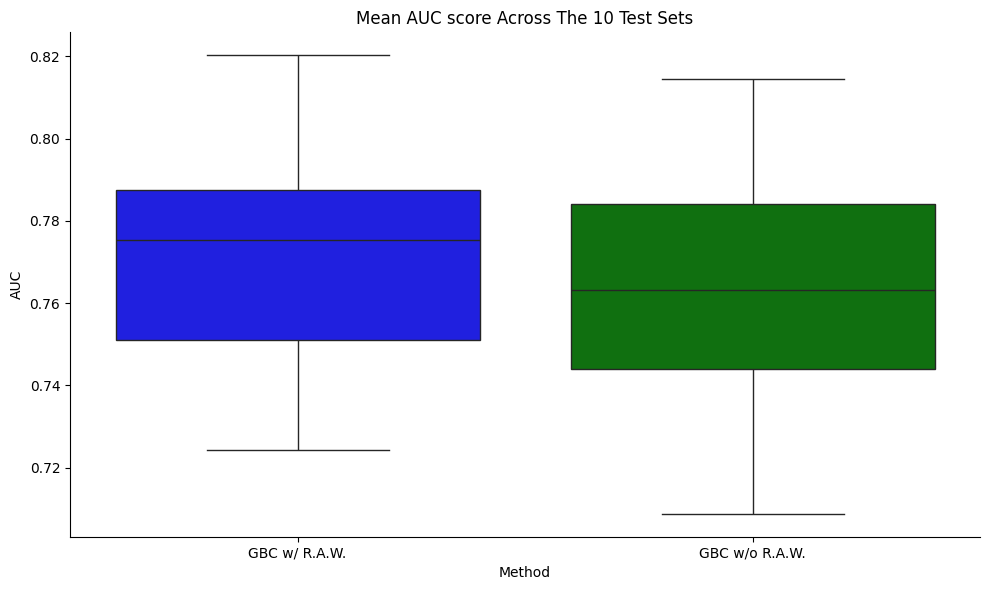
\includegraphics[width=0.8\textwidth]{assets/MeanAUCscoreacross10.png} 
    \caption{\textbf{Model Performance over Shifted Test Sets.}}
\end{figure}

To test the significance of the improvement, we conducted a Student's t-Test. The null hypothesis $\boldsymbol{H_0}$ is that the difference between the averaged AUC scores of model with and without R.A.W. is zero. The alternative hypothesis $\boldsymbol{H_1}$ is that this difference is not zero. The results of the t-Test are shown in the table below:

\begin{table}[H]
    \centering
    \begin{tabular}{lcccc}
        \toprule
        & $\Delta_{AUC}$ & t-stat & p-value & 95\% CI \\
        \midrule
        $\Delta_{\overline{\text{AUC}}}$ & 0.0083 & 8.75  & $1.39 \times 10^{-11}$ & [0.006, 0.010] \\
        \bottomrule
    \end{tabular}
\end{table}

Although the improvement is relatively small, the t-Test results show that the improvement is statistically significant.

\begin{figure}[H]
    \centering
    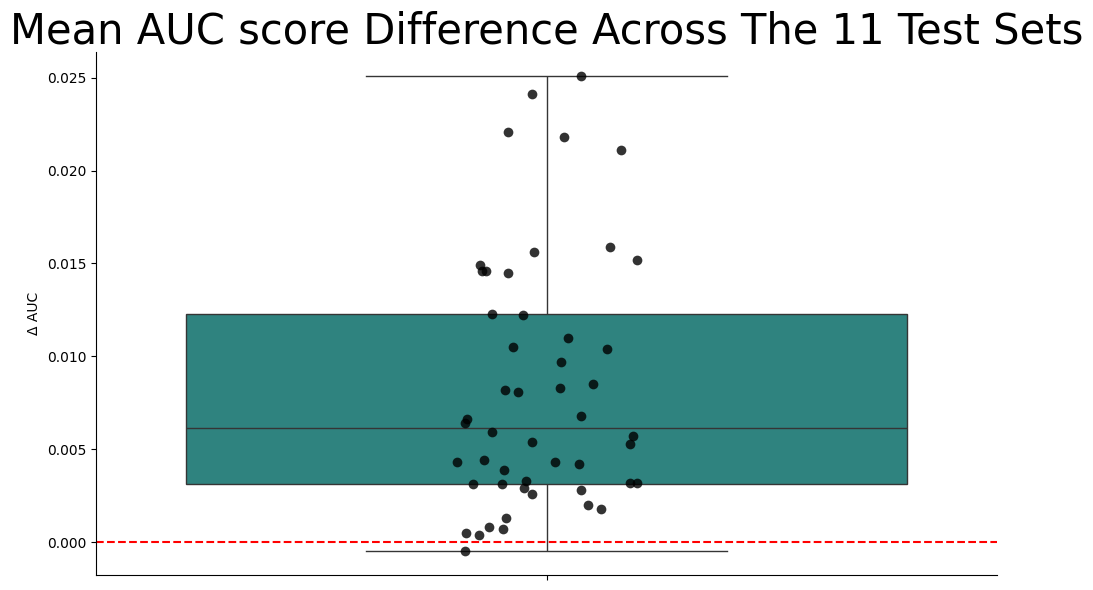
\includegraphics[width=0.8\textwidth]{assets/diffAUC10.png} 
    \caption{\textbf{50 AUC score differences between the baseline and augmented models.}Note that the difference is computed on the average AUC score across 11 test sets.}
\end{figure}


During the experiment, we also observed that the improvement in the model's performance is more pronounced when evaluated on the most shifted test set, i.e. the statistical mixture which does not include any datapoints from the non-shifted dataset:

\begin{figure}[H]
    \centering
    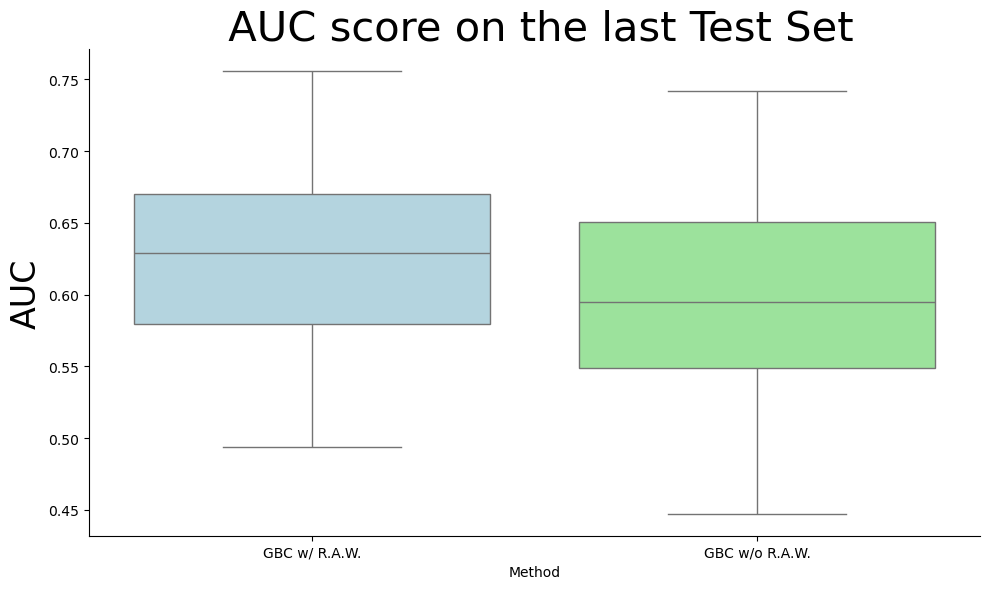
\includegraphics[width=0.8\textwidth]{assets/MeanAUCscoreLAST.png} 
    \caption{\textbf{Model Performances on the Most Shifted Test Set.}}
\end{figure}

A second t-Test was conducted on the differences in AUC scores in the 50 instances of this last test set:


\begin{table}[H]
    \centering
    \begin{tabular}{lcccc}
        \toprule
        & $\Delta_{AUC}$ & t-stat & p-value & 95\% CI \\
        \midrule
        $\Delta_{\text{AUC}_{\text{last}}}$ & 0.0235 & 10.59 & $2.86 \times 10^{-14}$ & [0.019, 0.028] \\
        \bottomrule
    \end{tabular}
\end{table}

The results highlight an increased improvement in the augmented model's performance when evaluated on the most shifted (and thus difficult) test set. 

\begin{figure}[H]
    \centering
    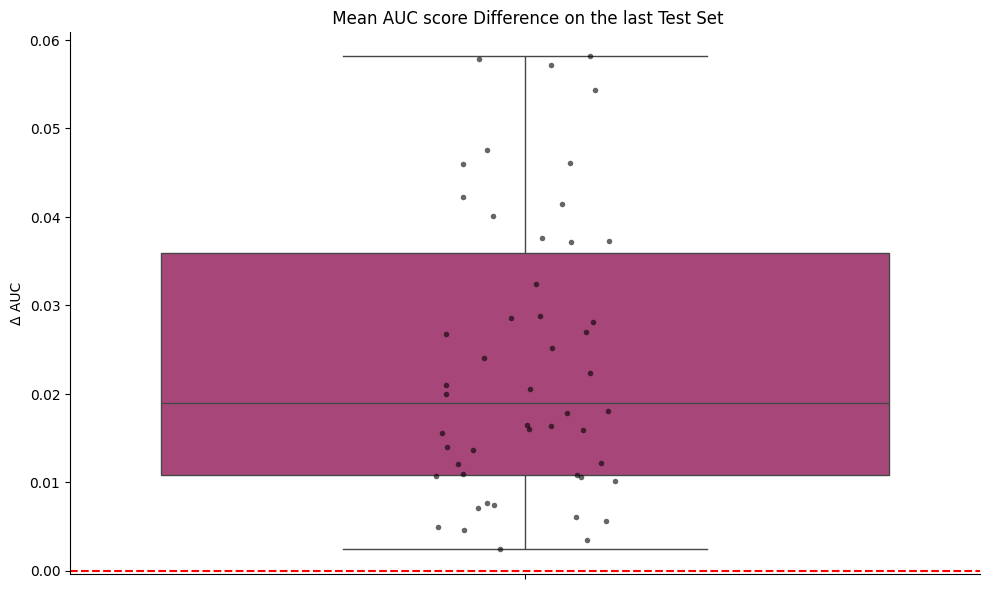
\includegraphics[width=0.8\textwidth]{assets/meandiffLAST.png} 
    \caption{\textbf{50 AUC score differences between the baseline and augmented models.}Note that the difference is computed on the AUC score of the last test set.}
\end{figure}

Lastly, we ran other 50 iterations of the experiment, this time we defined the covariance matrix used in the generation of the shifted sets as:

$$
[\boldsymbol{\Sigma}_{\text{shift}}]_{i,j} \sim \mathcal{U}_{[-0.75,0.75]} \text{for} i, j = 1, 2, 3
$$

Effectively increasing the range of the Uniform distribution used to generate the covariance matrix. The results of this experiment are shown in the figure below:

\begin{figure}[H]
    \centering
    \begin{subfigure}{0.45\textwidth}
        \centering
        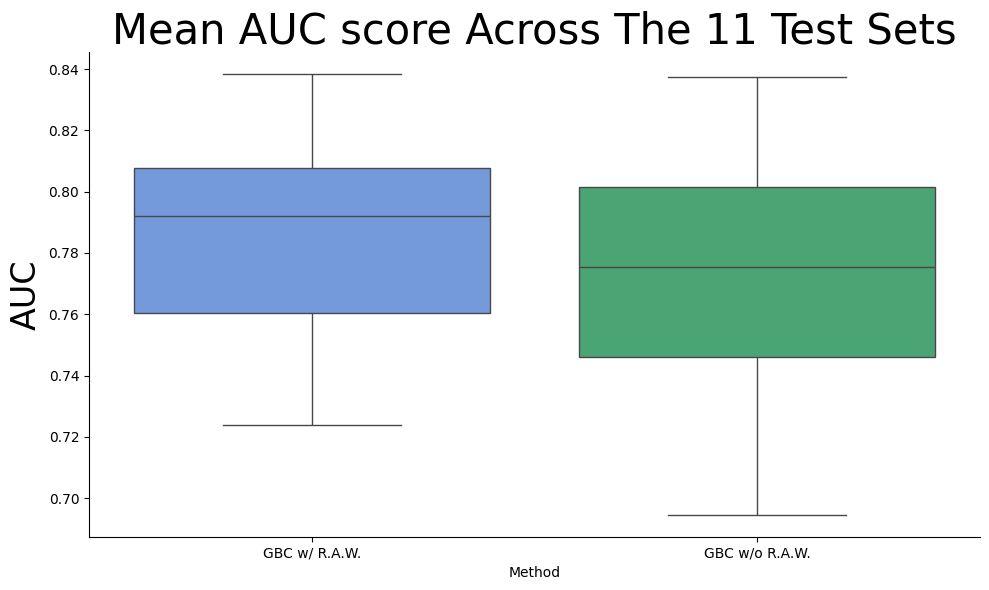
\includegraphics[width=\linewidth]{assets/1_075.png}
       
    \end{subfigure}
    \begin{subfigure}{0.45\textwidth}
        \centering
        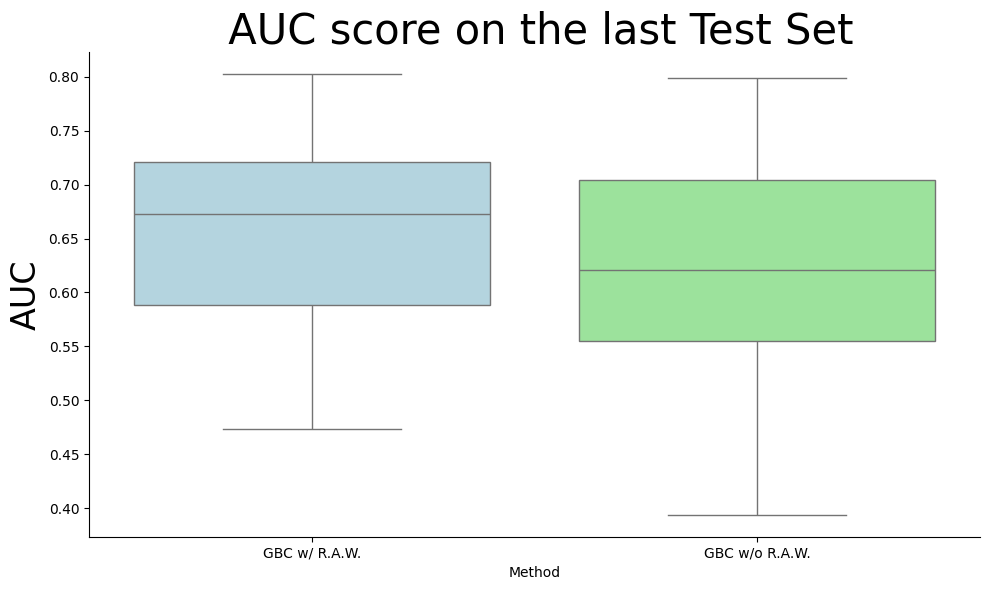
\includegraphics[width=\linewidth]{assets/2_075.png}
       
    \end{subfigure}
    \begin{subfigure}{0.45\textwidth}
        \centering
        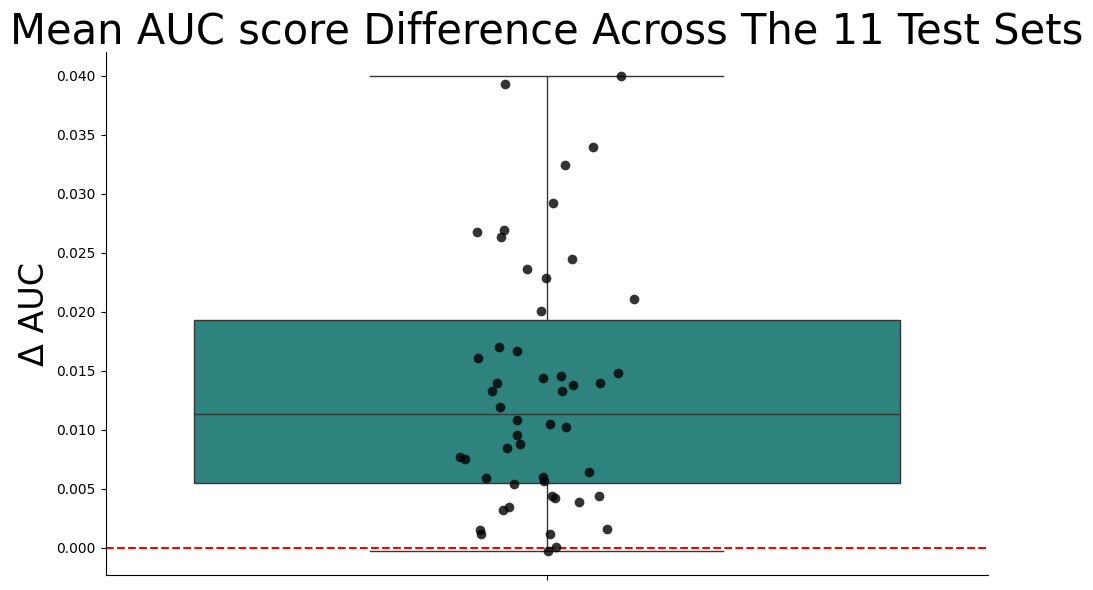
\includegraphics[width=\linewidth]{assets/3_075.png}
        
    \end{subfigure}
    \begin{subfigure}{0.45\textwidth}
        \centering
        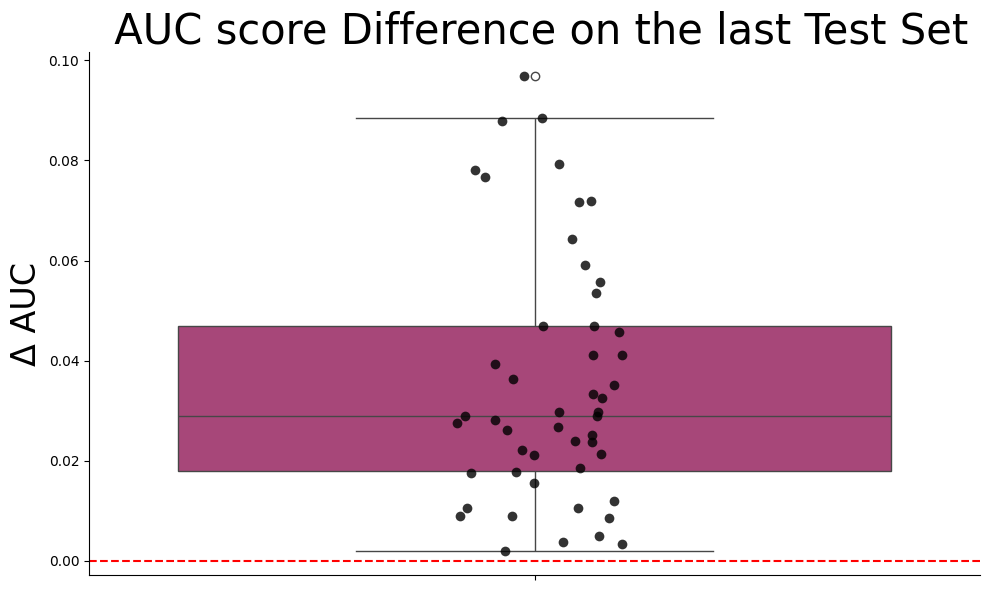
\includegraphics[width=\linewidth]{assets/4_075.png}
        
    \end{subfigure}
    \caption{\textbf{Model Performance with Increased Covariance Matrix shift.} Results when increasing the range of the uniform distribution used to generate the covariance matrix of shifted test sets. Note that the quantities of the y-axis are the same as the ones in the last experiment.}
\end{figure}


The results show that the improvement in the model's performance is more pronounced when the range of values in the covariance matrix is allowed to be large.
We conducted the same t-Tests as before, and the results are shown in the table below:

\begin{table}[H]
    \centering
    \small
    \begin{tabular}{lcccc}
        \toprule
        & $\Delta_{AUC}$ & t-stat & p-value & 95\% CI \\
        \midrule
        $\Delta_{\overline{\text{AUC}}}$ & 0.0135 & 9.2261  & $2.71 \times 10^{-12}$ & [0.011, 0.016] \\
        $\Delta_{\text{AUC}_{\text{last}}}$ & 0.0358 & 10.21 & $1.01 \times 10^{-13}$ & [0.029, 0.043] \\
        \bottomrule
    \end{tabular}
\end{table}




\subsection{Regression Task}

A 1-dimensional regression problem is considered to evaluate the performance of the Random Augmentation Walk method. The experiment is conducted as follows:

\subsubsection{Training Set}
The training set consists of 10,000 data points generated with $x$ values linearly spaced between -3 and 3, and $y$ values generated with the following formula:
\begin{equation}
    y = \sin(x)\exp(-x^2) + \varsigma
\end{equation}

Where $\varsigma$ is a random noise term drawn from a normal distribution with mean 0 and standard deviation 0.1.

\begin{figure}[H]
    \centering
    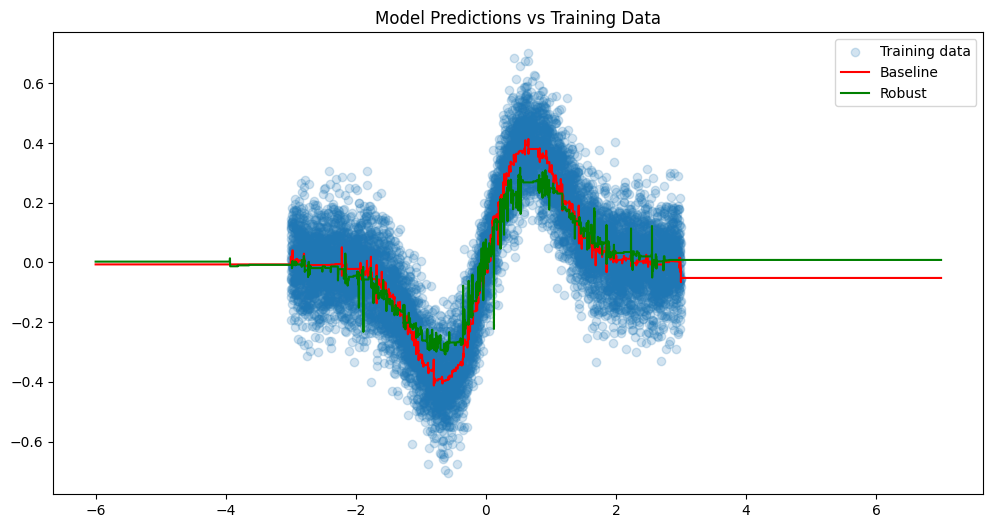
\includegraphics[width=0.8\textwidth]{assets/fit_on_train.png} 
    \caption{\textbf{Baseline and augmented models fit on the training data} To note that the augmented model has a \textbf{looser fit} on the training data.}
    \label{fig:fit-train}
\end{figure}

\subsubsection{Test Sets}
Thirty test sets are created by shifting the $x$ values by factors ranging from 1.5 to 5.5. Each shifted test set is generated independently using the same underlying function and noise process as the training data.
\begin{figure}[H]
    \centering
    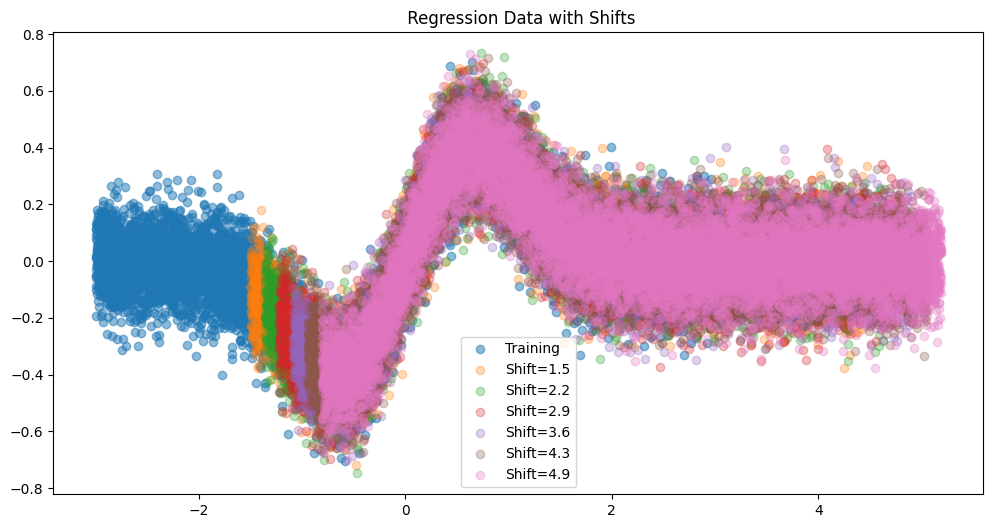
\includegraphics[width=0.8\textwidth]{assets/reg_shift_plot.png} 
    \caption{\textbf{A handful of test sets depicted together with the training set}}
    \label{fig:reg-shift-plot}
\end{figure}

\subsubsection{Models}
Two instances of the same model are trained with and without the Random Augmentation Walk method. The models are configured as follows:
\begin{itemize}
    \item \textbf{Baseline Model}: A Gradient Boosting Regressor (GBR) is employed as a baseline model. The GBR is configured with the following hyperparameters: \plaintt{n\_estimators=100, max\_depth=5, learning\_rate=0.05}.
    \item \textbf{R.A.W. Model}: This model has the same features as the baseline GBR but leverages the key parameters of the custom data augmentation method. The percentage of training data $N$ to be augmented is set to 40\%. Meanwhile the $\varepsilon$ which controls the magnitude of shifts considered in training is set to 1.
\end{itemize}


\subsection{Regression Results}

\subsubsection{Evaluation Metric}
The model performance is evaluated using the Mean Squared Error (MSE). For each shifted test set, the MSE is computed for both the baseline and augmented models.
The improvement is defined as the relative reduction in MSE computed as :
\begin{equation}
    \text{Improvement} = \left(\frac{\text{MSE}_{\text{baseline}} - \text{MSE}_{\text{aug}}}{\text{MSE}_{\text{baseline}}}\right) \times 100\%
\end{equation}

The metric is computed for each shift, and the results are shown in the figure below.
\begin{figure}[H]
    \centering
    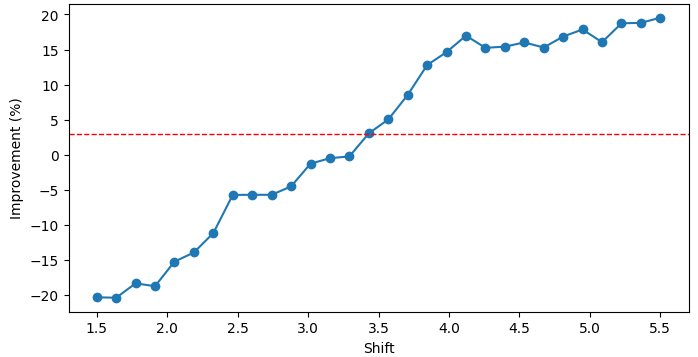
\includegraphics[width=0.8\textwidth]{assets/reg_exp_improvement.png} 
    \caption{\textbf{Model Improvement over Shifted Test Sets.} The red dotted line is the mean improvement across all shifts.}
    \label{fig:improv-plot}
\end{figure}

As we can see from the plot, the augmented model has worse performance then the baseline model for relatively small shifts but as the shift in data points becomes more significant, the augmented model outperforms the baseline model. The mean improvement across all shifts is still positive.
We believe the promising results of this methods are still to be analyzed in depth, but the preliminary results are encouraging.
